\documentclass[tikz,border=3pt]{standalone}
\usepackage{fontspec}
\usepackage{amsmath}
\usepackage{xcolor}
\usepackage{tikz}
\usepackage{pgfplots}
\pgfplotsset{compat=1.18}
\usetikzlibrary{arrows.meta,calc,fit,positioning,shapes.geometric,shapes.misc,patterns,plotmarks}
\IfFontExistsTF{Arial}{\setsansfont{Arial}}{\setsansfont{TeX Gyre Heros}}
\renewcommand{\familydefault}{\sfdefault}
\tikzset{
  >={Stealth[length=2.2mm,width=1.5mm]},
  exact title/.style={font=\bfseries\fontsize{10.5}{12}\selectfont,align=center},
  exact subtitle/.style={font=\fontsize{6.3}{7.2}\selectfont,align=center},
  exact label/.style={font=\fontsize{6.4}{7.5}\selectfont,align=center},
  exact tiny/.style={font=\fontsize{5.3}{6.3}\selectfont,align=center},
  panel/.style={draw=black!14,rounded corners=1.2mm,fill=white,line width=.45pt},
  neutral/.style={draw=black!30,fill=black!3,rounded corners=1mm,line width=.45pt},
  arrow/.style={-Stealth,line width=.7pt},
  softarrow/.style={-Stealth,line width=.55pt,draw=black!45},
  dashedarrow/.style={-Stealth,dashed,line width=.55pt,draw=black!55},
  metric/.style={font=\fontsize{5.3}{6.3}\selectfont,fill=white,inner sep=1pt},
}
\newcommand{\pill}[4]{\node[draw=#2!70,fill=#2!10,rounded corners=1.5mm,inner xsep=3pt,inner ysep=2pt,exact label,text=#2] (#1) at #3 {#4};}
\newcommand{\frameboxx}[4]{\draw[draw=#2!65,fill=#2!8,rounded corners=.6mm,line width=.5pt] (#1.south west) rectangle (#1.north east);\node[exact tiny,text=#2] at #3 {#4};}
\newcommand{\axislabel}[3]{\node[exact tiny,text=black!60] at (#1) {#2};\node[exact tiny,text=black!60,rotate=90] at (#3) {#2};}

\definecolor{nblue}{HTML}{2463A6}\definecolor{ngreen}{HTML}{2A9D8F}\definecolor{norange}{HTML}{F4A261}\definecolor{nink}{HTML}{1F2937}\definecolor{nmuted}{HTML}{E8EEF4}
\begin{document}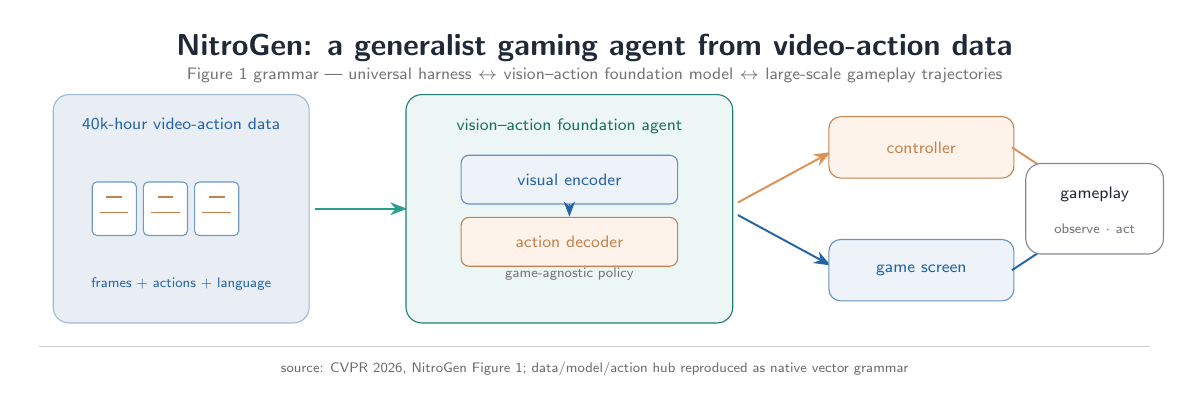
\begin{tikzpicture}[x=1cm,y=1cm]
\path[use as bounding box] (-.2,-2.3) rectangle (14.2,2.3);
\node[exact title,text=nink] at (7,2.04) {NitroGen: a generalist gaming agent from video-action data};
\node[exact subtitle,text=black!54] at (7,1.7) {Figure 1 grammar — universal harness \(\leftrightarrow\) vision–action foundation model \(\leftrightarrow\) large-scale gameplay trajectories};
\node[draw=nblue!45,fill=nmuted,rounded corners=2mm,minimum width=3.25cm,minimum height=2.9cm] (data) at (1.75,0) {};
\node[exact label,text=nblue] at (1.75,1.08) {40k-hour video-action data};
\foreach \x/\y in {.9/0,1.55/0,2.2/0}{\draw[nblue!65,fill=white,rounded corners=.6mm] (\x-.28,\y-.34) rectangle (\x+.28,\y+.34);\draw[norange!80!black,line width=.5pt] (\x-.18,\y-.05) -- (\x+.18,\y-.05);\draw[norange!80!black,line width=.5pt] (\x-.1,\y+.15) -- (\x+.1,\y+.15);}
\node[exact tiny,text=nblue] at (1.75,-.96) {frames + actions + language};
\draw[arrow,draw=ngreen] (3.45,0) -- (4.62,0);
\node[draw=ngreen!80!black,fill=ngreen!9,rounded corners=2mm,minimum width=4.15cm,minimum height=2.9cm] (model) at (6.68,0) {};
\node[exact label,text=ngreen!70!black] at (6.68,1.05) {vision–action foundation agent};
\node[draw=nblue!70,fill=nblue!8,rounded corners=1mm,minimum width=2.75cm,minimum height=.62cm,exact label,text=nblue] at (6.68,.37) {visual encoder};
\node[draw=norange!80!black,fill=norange!13,rounded corners=1mm,minimum width=2.75cm,minimum height=.62cm,exact label,text=norange!80!black] at (6.68,-.42) {action decoder};
\draw[softarrow,draw=nblue] (6.68,.06) -- (6.68,-.1);\node[exact tiny,text=black!55] at (6.68,-.83) {game-agnostic policy};
\draw[arrow,draw=norange!90!black] (8.82,.08) -- (10.0,.72);\draw[arrow,draw=nblue] (8.82,-.08) -- (10.0,-.72);
\node[draw=norange!80!black,fill=norange!13,rounded corners=1.5mm,minimum width=2.35cm,minimum height=.78cm,exact label,text=norange!80!black] at (11.15,.78) {controller};
\node[draw=nblue!70,fill=nblue!8,rounded corners=1.5mm,minimum width=2.35cm,minimum height=.78cm,exact label,text=nblue] at (11.15,-.78) {game screen};
\draw[arrow,draw=norange!90!black] (12.3,.78) -- (13.15,.22);\draw[arrow,draw=nblue] (12.3,-.78) -- (13.15,-.22);
\node[draw=nink!55,fill=white,rounded corners=2mm,minimum width=1.75cm,minimum height=1.15cm] at (13.35,0) {};
\node[exact label,text=nink] at (13.35,.18) {gameplay};\node[exact tiny,text=black!55] at (13.35,-.25) {observe \(\cdot\) act};
\draw[black!20,line width=.45pt] (-.05,-1.75) -- (14.05,-1.75);
\node[exact tiny,text=black!58] at (7,-2.03) {source: CVPR 2026, NitroGen Figure 1; data/model/action hub reproduced as native vector grammar};
\end{tikzpicture}\end{document}
